\section{INTRODUCTION}
\label{INTRODUCTION}

Anomaly detection problems have a great importance in industrial applications, because anomalies usually represent faults, failures or the emergence of such. To detect these automatically, we propose deep learning algorithms for anomaly / fault detection and their classification. We develop an algorithm achieving Segmentation Defects classification Its performance will be examined on two different problems: anomaly detection in oil pipelines and fault detection on transmission system components. Both these systems can span over thousands of kilometers, which makes manual inspection very costly. How such computer vision techniques can be applied on an industrial scale is discussed in the following.

Transmission infrastructure, on the other hand, physically connects power sources and consumers extending over thousands of kilometers. Many different components exist, which is why maintaining power grids is a serious cost factor for transmission system operators (TSOs). Automated fault detection could potentially help to decrease costs. To use an automated visual system however, specific infrastructure first needs to be identified and segmented, to then perform any type of fault detection. Therefore, the proposed deep learning-based approach, to segment and identify faulty components (i.e. insulators) in handheld footage, will be tested regarding its viability. If a deep-learning based approach would prove reliable, drones could monitor equipment automatically.

The damage of pipelines that transport petroleum and gas products lead to severe environmental problems. Eliminating breakthroughs and their consequences is expensive. To avoid accidents, it is recommended to improve diagnostics quality and to increase the frequency of in-line-inspection (ILI) tools deployment. ILI tools, also referred to as pipeline inspection gauges (Fig.~\ref{ris:ili}), use Hall effect for measuring localized magnetic flux leakage intensity along the pipe wall. While moving along the pipe gauge inspects the wall and detects the magnetic field leaks.
\begin{figure}[ht]
	\center{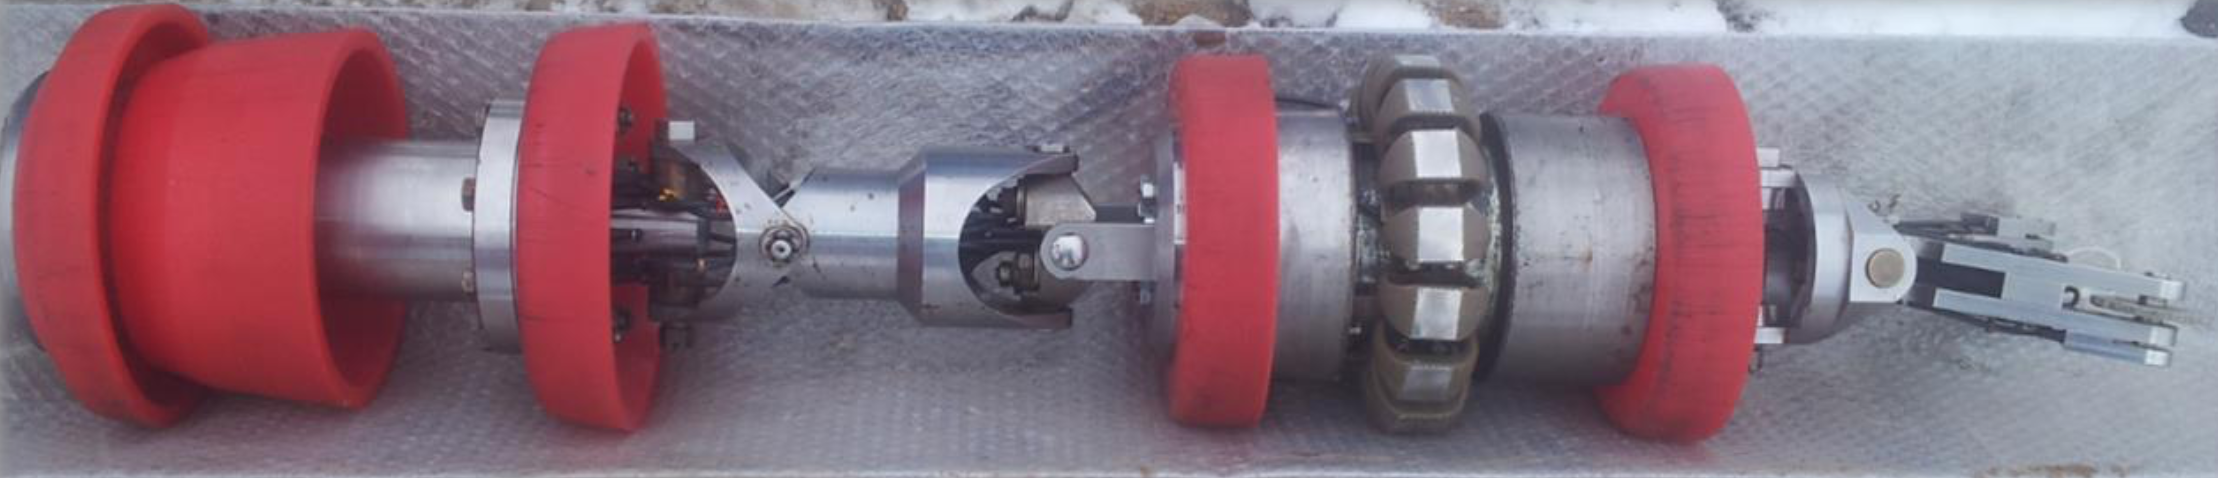
\includegraphics[scale=0.35]{pictures/ili.png}}
	\caption{In-line-inspection tool}
	\label{ris:ili}
\end{figure}
The data collected during the inspection can be further analyzed for main diagnostics problems solving: damage and defects detection, their localization, diagnosis or defects classification.
Analysis results are useful for assets managing and repair priorities determination.
